\subsection{Passeio Aleatório}
\begin{frame}[allowframebreaks]
  \frametitle{Caminhada do Bêbado}
        \begin{figure}[h!]
        \centering
        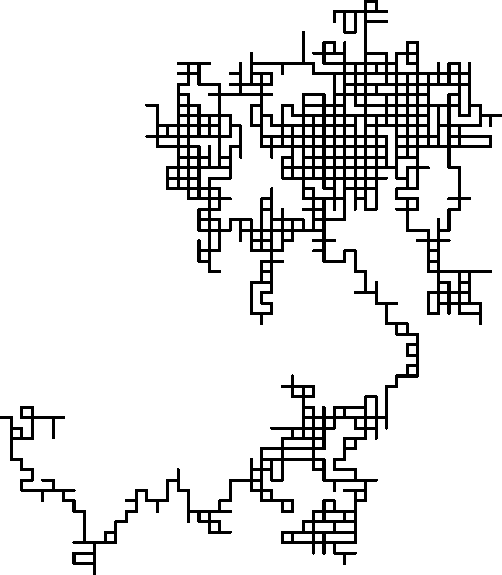
\includegraphics[width=0.25\textwidth]{images/randomwalk.pdf}
        \caption{Passeio aleatório (Wikipedia).}
        \label{fig:random_walk_2d}
        \end{figure}

  Vamos considerar aqui o exemplo do passeio aleatório sobre um grafo com pesos.
  \begin{itemize}
  \item Assuma uma distribuição estacionária irredutível e aperiódica.
  \item Considere o grafo $G=(V,E)$ com $m$ nós rotulados $\{1, 2, \ldots, m\}$ e arestas entre os nós com pesos $w_{ij} \geq 0$ 
	(aresta entre o nó $i$ e o nó $j$). Teremos $w_{ij} = w_{ji}$ e $w_{ij}=0$ se não existe aresta entre os nós $i$ e $j$.

        \begin{figure}[h!]
        \centering
        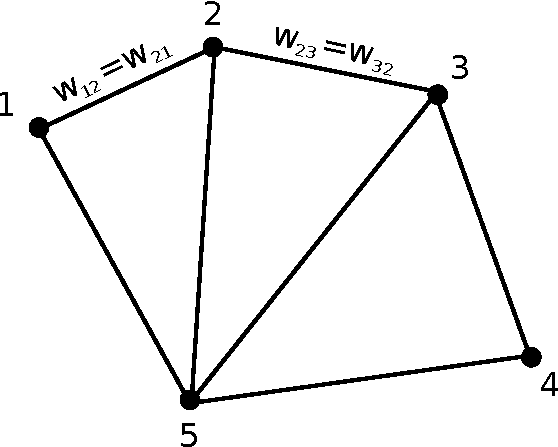
\includegraphics[width=0.3\textwidth]{images/grafo.pdf}
        \label{fig:grafo}
        \end{figure}

  \item O andar do bêbado (\textit{random walk}) $\{ X_n \}$, $X_n \in \{1,2,\ldots,m\}$, é uma sequência de vértices de um grafo.
  \item Dado $X_n = i$, o próximo vértice $j$ será escolhido dentre aqueles nós conectados com $i$ com probabilidade proporcional
	ao peso conectando os vértices $i$ e $j$, i.e., $p_{ij}$ será dado por
	\begin{equation}
	p_{ij} = \frac{w_{ij}}{\sum_j w_{ij}} = \frac{w_{ij}}{w_i}
	\end{equation}
	onde $w_i \triangleq \sum_j w_{ij}$ (peso total das arestas que saem do nó $i$).
  \item A soma de todos os pesos, de todas as arestas será dada por
	\begin{equation}
	w = \sum_{i,j : j > i} w_{ij}
	\end{equation}
  \item Note que $\sum_i w_i = \sum_{i,j} w_{ij} = 2w$.
  \item Vamos supor que a distribuição estacionária é dada por $\mu_i = \frac{w_i}{2w}$, o que poderemos
	checar verificando a equação $\mu^T = \mu^T P$:
	\begin{equation}
	\begin{pmatrix} \mu_1 & \mu_2 & \ldots & \mu_m \end{pmatrix} =  
		\begin{pmatrix} \mu_1 & \mu_2 & \ldots & \mu_m \end{pmatrix}
 		\begin{pmatrix}
		p_{11} & p_{12} & \ldots & p_{1m} \\
		p_{21} & p_{22} & \ldots & p_{2m} \\
		\vdots & \vdots & \ddots & \vdots \\
		p_{m1} & p_{m2} & \ldots & p_{mm}
		\end{pmatrix}
	\end{equation}
	ou seja,
	\begin{equation}
	\forall j, \quad \sum_i \mu_i p_{ij} = \sum_i \frac{w_i}{2w} \frac{w_{ij}}{w_i} = \sum_i \frac{1}{2w} w_{ij} = \frac{w_j}{2w} = \mu_j
	\end{equation}
  \item $\mu_j = \frac{w_j}{2w}$ : esta distribuição estacionária possui uma interessante propriedade de localização:
	ela depende apenas dos pesos locais (conectados ao nó em questão) e do total dos pesos; desta forma, ela não 
	sofrerá alteração se os pesos de uma outra parte do grafo (com arestas não ligadas ao nó $i$) 
	sofrerem alteração sem alterar a soma dos pesos.
  \item Note que a cadeia é aperiódica, já que $w_{ii} = 0$, como evidenciado abaixo
	\begin{eqnarray}
	2w &=& \sum_i w_i = \sum_{i,j} w_{ij} = \sum_{i,j : i=j} w_{i,j} + \sum_{i,j : i>j} w_{i,j} + \sum_{i,j : i<j} w_{i,j}  \nonumber \\
	&=& \sum_{i,j : i=j} w_{i,j} + w + w = \sum_{i,j : i=j} w_{i,j} + 2w
	\end{eqnarray}
 	logo, $\sum_{i,j : i=j} w_{i,j} = 0 \Rightarrow w_{ii} = 0$.
  \item A taxa de entropia para este passeio aleatório será dada por
	\begin{eqnarray}
	H(\mathcal{X}) &=& H(X_2 \mid X_1) = -\sum_i \mu_i \sum_j p_{ij} \log p_{ij} \nonumber \\
		&=& - \sum_i \frac{w_i}{2w} \sum_j \frac{w_{ij}}{w_i} \log \frac{w_{ij}}{w_i} = - \sum_{i,j} \frac{w_{ij}}{2w} \log \frac{w_{ij}}{w_i} \nonumber \\
		&=& - \sum_{i,j} \frac{w_{ij}}{2w} \log \left( \frac{w_{ij}}{w_i} \frac{2w}{2w} \right) \nonumber \\
		&=& - \sum_{i,j} \frac{w_{ij}}{2w} \log \frac{w_{ij}}{2w} - \sum_{i,j} \frac{w_{ij}}{2w} \log \frac{2w}{w_i} \nonumber \\
		&=& H\left( \ldots,\frac{w_{ij}}{2w} , \ldots \right) - H\left( \ldots,\frac{w_{i}}{2w} , \ldots \right) 
	\end{eqnarray}
	onde o primeiro termo representa a incerteza sob todas arestas e o segundo termo representa a incerteza sob todos os nós em condição estacionária
	($w_i/2w=\mu_i$).

	Se todas arestas possuírem o mesmo peso, sendo $E_i$ o número de arestas emanando do nó $i$, e $E$
	o número total de arestas, teremos
	\begin{equation}
	H(\mathcal{X}) = \log (2E) - H \left( \frac{E_1}{2E}, \frac{E_2}{2E}, \ldots, \frac{E_m}{2E} \right) .
	\end{equation}
  \end{itemize}
\end{frame}


\subsection{Cadeia Oculta de Markov}
\begin{frame}[allowframebreaks]
  \frametitle{Modelo de Markov}
        \begin{figure}[h!]
        \centering
        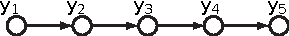
\includegraphics[width=0.4\textwidth]{images/mm.pdf}
        \label{fig:mm}
        \end{figure}
  Para o modelo de Markov de primeira ordem, temos que dois estados são independentes quando um intermediário é dado, por exemplo:
	\begin{equation}
	Y_5 \independent Y_3 \mid Y_4 \text{ ou então } Y_4 \independent Y_1 \mid Y_{2:3} \text{ ou } Y_4 \independent Y_1 \mid Y_2
	\end{equation}
\end{frame}


\begin{frame}[allowframebreaks]
  \frametitle{Cadeia Oculta Markov}
        \begin{figure}[h!]
        \centering
        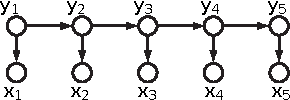
\includegraphics[width=0.4\textwidth]{images/hmm.pdf}
        \label{fig:hmm}
        \end{figure}
  Na cadeia oculta de Markov, dizemos que um observação é gerada por um estado independente de outras observações ou estados passados.
  Por exemplo:
	\begin{equation}
        X_3 \independent X_1 \mid Y_3
        \end{equation}

  \framebreak

  \begin{itemize}
  \item Seja $Y_1, Y_2, \ldots, Y_n$ uma cadeia de Markov estacionária.
  \item Seja $X_{1:n}$ uma função aleatória desta cadeia de Markov, i.e.,
	\begin{equation}
	X_i = \phi_N (Y_i) = \begin{cases}
				\phi_1 (Y_i) \quad \text{com prob. } p_1(Y_i) \\
				\phi_2 (Y_i) \quad \text{com prob. } p_2(Y_i) \\
				\vdots \\
				\phi_m (Y_i) \quad \text{com prob. } p_m(Y_i) 
				\end{cases}
	\end{equation}
	onde $N \in \{1,2,\ldots,m\}$ é uma variável aleatória.
  \item Note que o processo estocástico $X_1,X_2,\ldots$ não forma uma cadeia de Markov. Sequer a Markovidade de primeira ordem é satisfeita.
	Por exemplo: não podemos falar que $X_4 \independent X_1 \mid X_{2:3}$, 
	mesmo conhecendo $X_{2:3}$, $X_1$ ainda pode ser necessário para determinar $X_4$.
  \item Se $\{Y_i\}_i$ é estacionário, então $\{X_i\}_i$ é um processo estacionário.
  \item A taxa de entropia do processo $\{X_i\}_i$ pode ser calculada
	\begin{equation}
	H(\mathcal{X}) = \lim_{n \rightarrow \infty} H(X_n \mid X_{n-1}, \ldots, X_1) 
	\end{equation}
	mas iremos calcular os limites inferior e superior, o que é mais simples.
  \item Limite superior:
	\begin{eqnarray}
	H(X_n \mid X_{n-1}, \ldots, X_1) &=& H(X_{n+1} \mid X_{n}, \ldots, X_2) \nonumber \\
		&\geq& H(X_{n+1} \mid X_{n}, \ldots, X_2, X_1) \nonumber \\
		&=& H(X_{n+2} \mid X_{n+1}, \ldots, X_2) \nonumber \\
		&\geq& H(X_{n+2} \mid X_{n+1}, \ldots, X_2, X_1) \nonumber \\
		&\geq& \ldots \geq H(\mathcal{X})
	\end{eqnarray}
  \item Limite inferior:
	\begin{eqnarray}
	H(X_n \mid X_{n-1}, \ldots, X_2, Y_1) = H(X_n \mid X_{n-1}, \ldots, X_2, X_1,Y_1) \nonumber \\
		\text{já que } X_n \independent X_1 \mid Y_1 \nonumber \\
		= H(X_n \mid X_{n-1}, \ldots, X_2, X_1,Y_1,Y_0,Y_{-1},\ldots,Y_{-k}) \\
		\text{já que } X_n \independent Y_0 \mid Y_1 \text{ e } X_n \independent Y_{-1} \mid Y_1 \text{ etc...} \nonumber \\
		= H(X_n \mid X_{n-1}, \ldots, X_2, X_1,Y_1,Y_0,Y_{-1},\ldots,Y_{-k},X_0,\ldots,X_{-k}) \nonumber \\
		\text{pelo mesmo motivo} \nonumber \\
		\leq H(X_n \mid X_{n-1}, \ldots, X_2, X_1,X_0,\ldots,X_{-k}) \nonumber \\
		\text{condicionar reduz a entropia} \nonumber \\
		= H(X_{n+k+1} \mid X_{n+k}, \ldots, X_1) \\
		\text{estacionariedade} \nonumber 
	\end{eqnarray}
 	Desta forma temos o limite inferior:
	\begin{equation}
	H(X_n \mid X_{n-1}, \ldots, X_2, Y_1) \leq H(\mathcal{X})
	\end{equation}
  \item Os limites para a taxa de informação em uma HMM são dados 
	\begin{equation}
        H(X_n \mid X_{n-1}, \ldots, X_1, Y_1) \leq H(\mathcal{X}) \leq H(X_n \mid X_{n-1}, \ldots, X_1)
	\end{equation}
  \end{itemize}


  \framebreak

  \begin{theorem}[teorema do confronto (sanduíche)]
  \begin{equation}
  H(X_n \mid X_{n-1}, \ldots , X_1) - H(X_n \mid X_{n-1}, \ldots, X_1, Y_1) \rightarrow 0
  \end{equation}
  \end{theorem}

  \begin{proof}
  \begin{eqnarray}
  H(X_n \mid X_{n-1}, \ldots , X_1) - H(X_n \mid X_{n-1}, \ldots, X_1, Y_1)  \nonumber \\
	= I(X_n ; Y_1 \mid X_{n-1}, \ldots, X_1) \leq H(Y_1)
  \end{eqnarray}
  Temos também que $I(Y_1 ; X_1, \ldots, X_n) \leq H(Y_1)$, para todo $n$.
  \proofbreak
  Utilizando a regra da cadeira da informação mútua ($I(X;Y,Z) = I(X;Z) + I(X;Y|Z)$), e tirando o limite, teremos
  \begin{eqnarray}
  \lim_{n \rightarrow \infty} I(Y_1 ; X_1, \ldots, X_n) =  \lim_{n \rightarrow \infty} \sum_{i=1}^n I(Y_1;X_i \mid X_{1:i-1}) \nonumber \\
	= \sum_{i=1}^\infty I(Y_1;X_i \mid X_{1:i-1}) \leq H(Y_1) < \infty
  \end{eqnarray} 
  Então o resultado da soma infinita é uma constante, isto significa que os termos $\rightarrow 0$ quando $n \rightarrow \infty$.
  Logo, cada um dos termos $I(Y_1;X_i \mid X_{1:i-1}) \rightarrow 0$ quando $n \rightarrow \infty$.
  \end{proof}

  \framebreak

  Ao final, temos que
  \begin{equation}
  \lim_{n \rightarrow \infty} H(X_n \mid X_{n-1}, \ldots, X_1, Y_1) = H(\mathcal{X}) = \lim_{n \rightarrow \infty} H(X_n \mid X_{n-1}, \ldots, X_1)
  \end{equation}
\end{frame}


\subsection{Modelos de Ehrenfest}
\begin{frame}[allowframebreaks]
  \frametitle{Modelos de Ehrenfest}

Paul Ehrenfest propôs um modelo simples para a troca de calor ou moléculas entre
dois corpos isolados. Neste modelo da cadeia de Ehrenfest iremos considerar a troca de
moléculas de gás entre dois compartimentos, rotulados por 0 e 1,
conforme apresentado na Figura \ref{fig:ehrenfes}.

\begin{figure}[h]
  \centering
  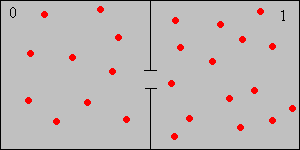
\includegraphics[width=0.25\textwidth]{images/ehrenfest.png}
  \caption{Modelo de Ehrenfest.}
  \label{fig:ehrenfes}
\end{figure}

Iremos denotar por $X_k$ o número de partículas no compartimento 1 no instante $k$.
$X_k$ descreve o estado atual do sistema. Temos um processo estocástico gerando $X_{1:n}$,
onde $X_k \in \{0,1,\ldots,m\}$.

\framebreak 

Supondo que no instante $k$ o compartimento 1 possua $i$ partículas ($X_k = i$).
O modelo de Ehrenfest nos fornece:
\begin{eqnarray}
\Pr(X_{k+1} = i+1 | X_k = i) &=& \frac{m - i}{m} , \nonumber  \\
\Pr(X_{k+1} = i-1 | X_k = i) &=& \frac{i}{m} .
\end{eqnarray}

Neste modelo a propriedade de Markov é satisfeita:
\begin{eqnarray}
\Pr(X_{n+1} = i+1 | X_0 = i_0, X_1 = i_1, \ldots, X_{n-1} = i_{n-1}, X_n = i) &=& \Pr(X_{n+1} = i+1 | X_n = i) , \nonumber \\
\Pr(X_{n+1} = i-1 | X_0 = i_0, X_1 = i_1, \ldots, X_{n-1} = i_{n-1}, X_n = i) &=& \Pr(X_{n+1} = i-1 | X_n = i) . \nonumber
\end{eqnarray}
A distribuição condicional não depende de $n$, desta forma, temos um processo estocástico homogêneo. 
A cadeia de Markov poderá então ser descrita por uma matriz de transição fixa $P = [p_{ij}]_{ij}$.

\framebreak

Para $m = 4$ teremos a cadeia de Markov representada pelo grafo a seguir:
\begin{center}
\begin{tikzpicture}[->, >=stealth', auto, semithick, node distance=3cm]
\tikzstyle{every state}=[fill=white,draw=black,thick,text=black,scale=1]
\node[state]    (0)               {$0$};
\node[state]    (1)[right of=0]   {$1$};
\node[state]    (2)[right of=1]   {$2$};
\node[state]    (3)[right of=2]   {$3$};
\node[state]    (4)[right of=3]   {$4$};
\path
(0) edge[bend left,above]   node{$1$}    (1)
(1) edge[bend left,below]   node{$1/4$}  (0)
(1) edge[bend left,above]   node{$3/4$}  (2)
(2) edge[bend left,below]   node{$1/2$}  (1)
(2) edge[bend left,above]   node{$1/2$}  (3)
(3) edge[bend left,below]   node{$3/4$}  (2)
(3) edge[bend left,above]   node{$1/4$}  (4)
(4) edge[bend left,below]   node{$1$}    (3) ;
% edge[loop left]     node{$p^2$}         (1) ;
\end{tikzpicture}
\end{center}


\framebreak
\begin{equation}
\mathbf{P} = 
\begin{blockarray}{cccccc}
0 & 1 & 2 & 3 & 4 \\
\begin{block}{(ccccc)c}
  0   & 1   & 0   & 0   & 0   & 0 \\
  1/4 & 0   & 3/4 & 0   & 0   & 1 \\
  0   & 1/2 & 0   & 1/2 & 0   & 2 \\
  0   & 0   & 3/4 & 0   & 1/4 & 3 \\
  0   & 0   & 0   & 1   & 0   & 4 \\
\end{block}
\end{blockarray}
\end{equation}


\framebreak

A distribuição de estado estacionário é tal que $\mathbf{\mu}^T P = \mathbf{\mu}^T$, com $\sum_i \mu_i = 1$.

\begin{eqnarray}
\mathbf{\mu}^T P &=& \mathbf{\mu}^T \nonumber \\
\mathbf{\mu}^T (P-I) &=& 0 \nonumber \\
\mathbf{\mu}^T Q &=& 0 
\end{eqnarray}

Teremos aqui
\begin{equation}
Q = \begin{pmatrix} 
-1  &  1  & 0   & 0   & 0   \\
1/4 & -1  & 3/4 & 0   & 0   \\
0   & 1/2 & -1  & 1/2 & 0   \\
0   & 0   & 3/4 & -1  & 1/4 \\
0   & 0   & 0   & 1   & -1
\end{pmatrix} .
\end{equation}


\framebreak

Vamos incorporar a condição $\sum_i \mu_i = 1$ fazendo:
\begin{equation}
\tilde{Q} = \begin{pmatrix} 
-1  &  1  & 0   & 0   & 1 \\
1/4 & -1  & 3/4 & 0   & 1 \\
0   & 1/2 & -1  & 1/2 & 1 \\
0   & 0   & 3/4 & -1  & 1 \\
0   & 0   & 0   & 1   & 1
\end{pmatrix} ,
\end{equation}
e o novo sistema de equações será
\begin{equation}
\mathbf{\mu}^T \tilde{Q} = (0, 0, 0, 1) .
\label{eq-novo-sistema}
\end{equation}


\framebreak
Para solucionar a Equação \ref{eq-novo-sistema}, iremos pós multiplicar ambos os lados
pela matriz inversa de $\tilde{Q}$,
\begin{equation}
\mathbf{\mu}^T = (0, 0, 0, 1) \tilde{Q}^{-1} ,
\end{equation}
obtendo assim 
\begin{equation}
\mathbf{\mu}^T = \left( \frac{1}{16}, \frac{1}{4}, \frac{6}{16}, \frac{1}{4}, \frac{1}{16} \right)
\end{equation}


\framebreak

A taxa de entropia para um cadeia de Markov de primeira ordem
estacionária será dada da seguinte forma
  \begin{eqnarray}
  H(\mathcal{X}) &=& H'(\mathcal{X}) = \lim_{n \rightarrow \infty} H(X_n \mid X_{n-1}, \ldots, X_1) \nonumber \\
        &=& \lim_{n \rightarrow \infty} H(X_n \mid X_{n-1}) \nonumber \\
        && \text{dado que é Markov de 1a ordem} \nonumber \\
        &=& H(X_2 \mid X_1) \quad \text{(estacionário)} \nonumber \\
        &=& - \sum_{x_2, x_1} p(x_2, x_1) \log p(x_2 \mid x_1) = \sum_i \mu_i \left[ - \sum_j p_{ij} \log p_{ij} \right] \nonumber \\
        &=& \sum_i \mu_i H( \mathbf{p_i} )
  \end{eqnarray}
onde $\mu$ é a distribuição estacionária,
$p_{ij}$ a probabilidade de transição de $i$ para $j$ (elementos da matriz $P$)
e $\mathbf{p_i}$ a $i$-ésima linha da matriz $P$ (as probabilidades de transição à partir
do estado $i$).

\framebreak

Para o exemplo em questão:
\begin{eqnarray}
  H(\mathcal{X}) &=& \mu_1 H(\mathbf{p_1}) + \mu_2 H(\mathbf{p_2}) + \mu_3 H(\mathbf{p_3}) +
        \mu_4 H(\mathbf{p_4}) + \mu_5 H(\mathbf{p_5}) \nonumber \\
        &=& \frac{1}{16} H(0,1,0,0,0) + \frac{1}{4} H(\frac{1}{4}, 0, \frac{3}{4}, 0, 0) + 
                \frac{6}{16} H(0, \frac{1}{2}, 0, \frac{1}{2}, 0) + 
                \frac{1}{4} H(0, 0, \frac{3}{4}, 0, \frac{1}{4}) \nonumber \\
            && + \frac{1}{16} H(0, 0, 0, 1, 0) \nonumber \\
        &=& 0 + 2 \times \frac{1}{4} \left( \frac{1}{4} \log 4 + \frac{3}{4} \log \frac{4}{3} \right) +
                \frac{6}{16} + 0 \nonumber \\
        &=& \frac{1}{2} \left( \frac{1}{2} + \frac{3}{2} - \frac{3}{4} \log 3  \right) + \frac{6}{16} \nonumber \\
        &=& 1 - \frac{3}{8} \log 3 + \frac{6}{16} = \frac{11}{8} - \frac{3}{8} \log 3 = 0.78064
\end{eqnarray}


\end{frame}

